\chapter{Results}
\ldots\todo[inline]{3 pages}
\todo[inline]{some very nice graphs}

\section{Technical Details}
\begin{itemize}
  \item Intel\textsuperscript{\textregistered}~Core\texttrademark~2 Duo CPU E6850
  \item 2 GB RAM
  \item \todo[inline]{CGAL version}
\end{itemize}

\section{Segment Lengths}

\newgeometry{margin=1.5cm}
\begin{landscape}
\begin{figure}[ht]
  \centering
  \thisfloatpagestyle{empty}
  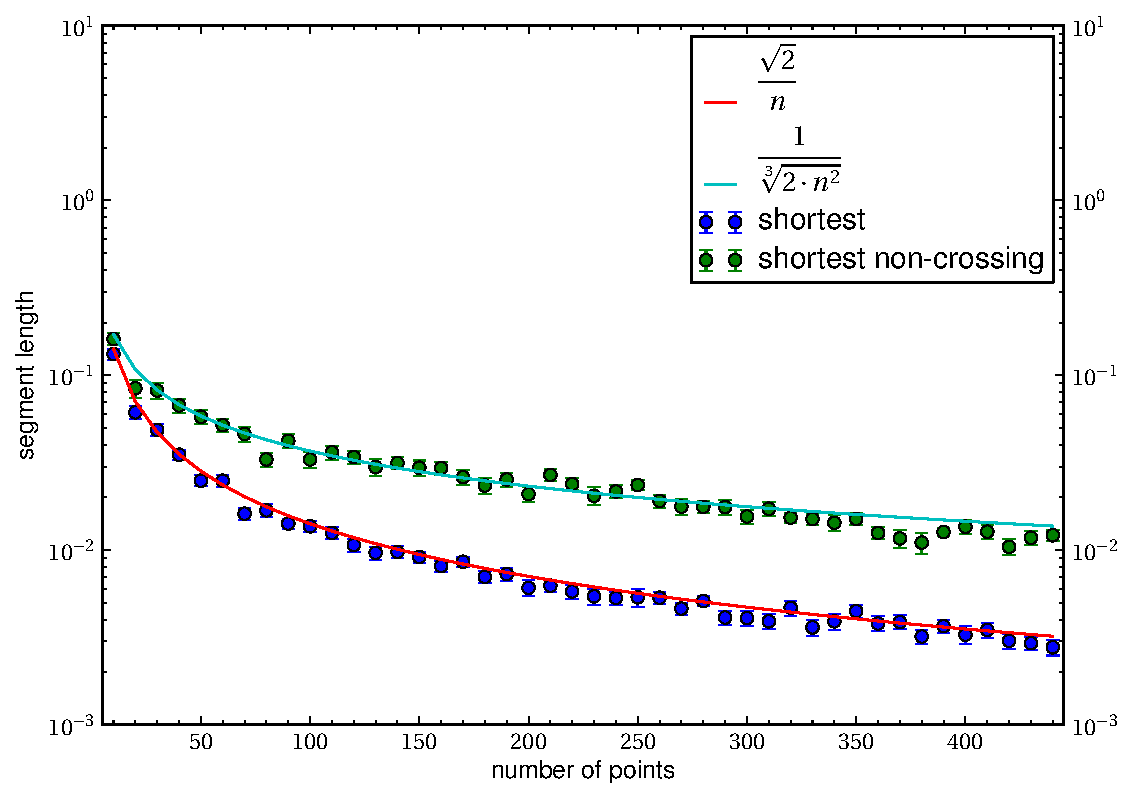
\includegraphics[width=\linewidth,keepaspectratio]{results/segment_length.pdf}
  \caption{\label{fig:segment_lengths}Comparison of segment lengths}
\end{figure}

\begin{figure}[ht]
  \centering
  \thisfloatpagestyle{empty}
  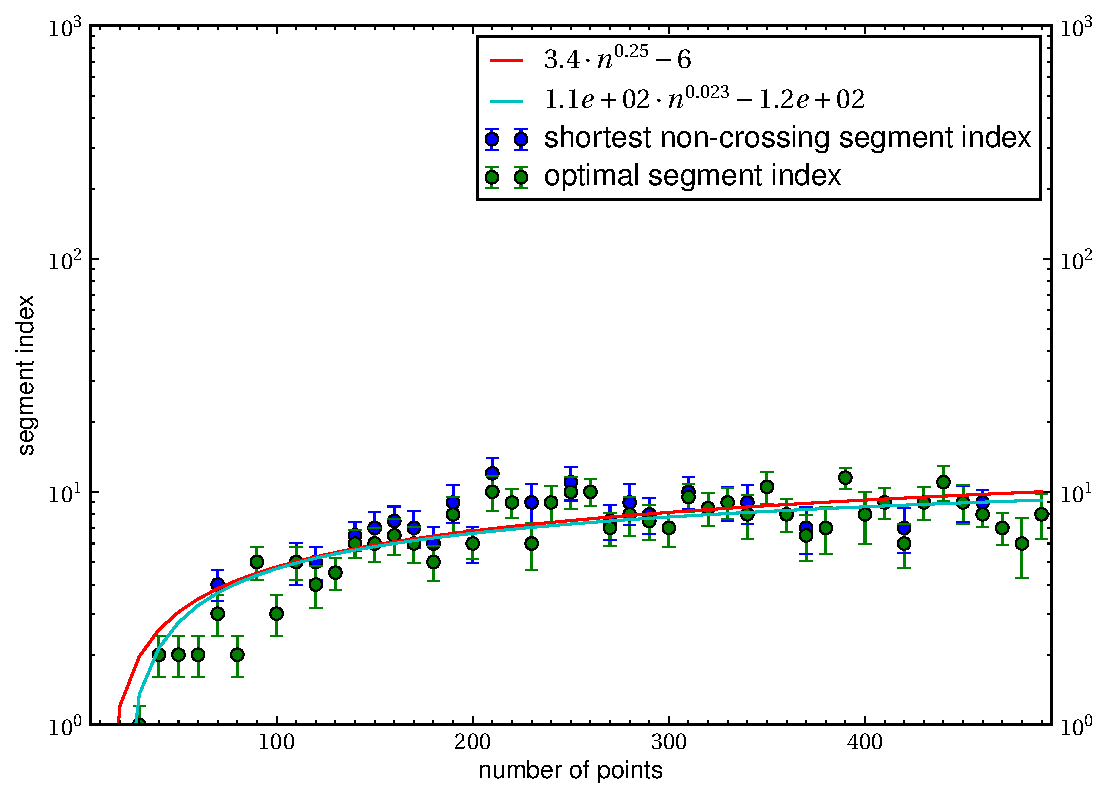
\includegraphics[width=\linewidth,keepaspectratio]{results/segment_index.pdf}
  \caption{\label{fig:segment_index}Comparison of segment indices}
\end{figure}
\end{landscape}
\restoregeometry

\section{Execution Time}

\newgeometry{margin=1.5cm}
\begin{landscape}
\begin{figure}[ht]
  \centering
  \thisfloatpagestyle{empty}
  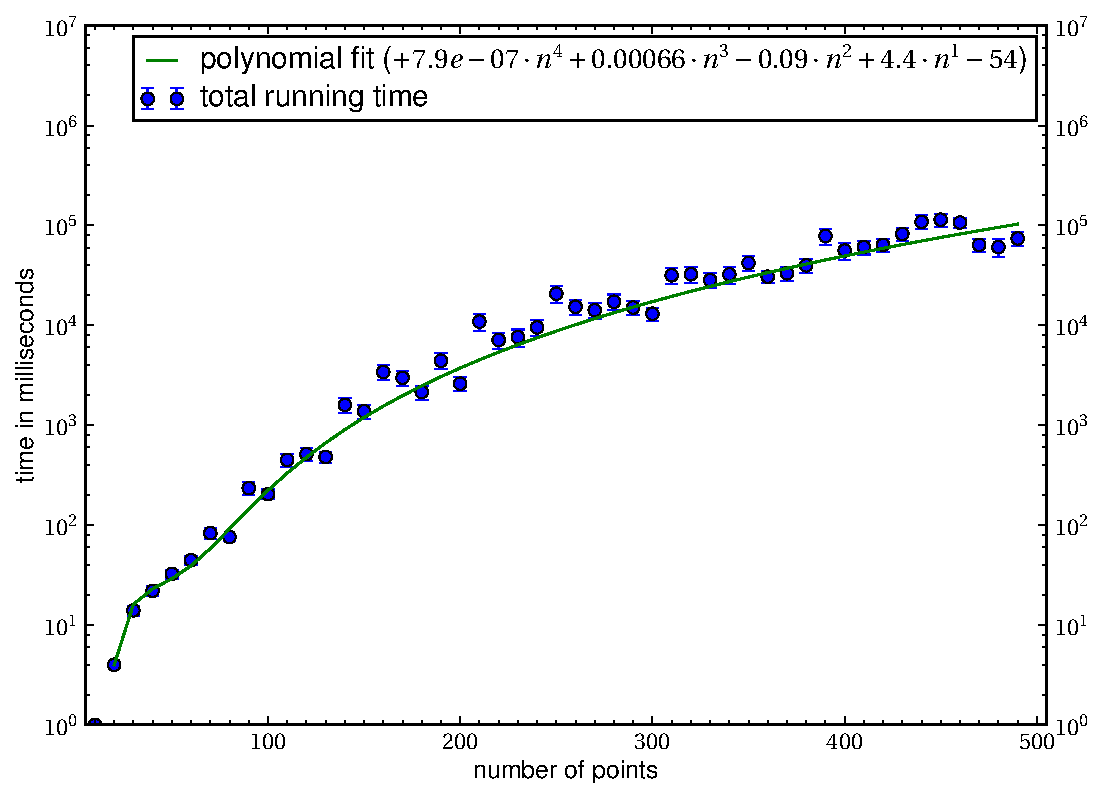
\includegraphics[width=\linewidth,height=\textheight,keepaspectratio]{results/time_total.pdf}
  \caption{\label{fig:time_total}Total execution time}
\end{figure}

\begin{figure}[ht]
  \centering
  \thisfloatpagestyle{empty}
  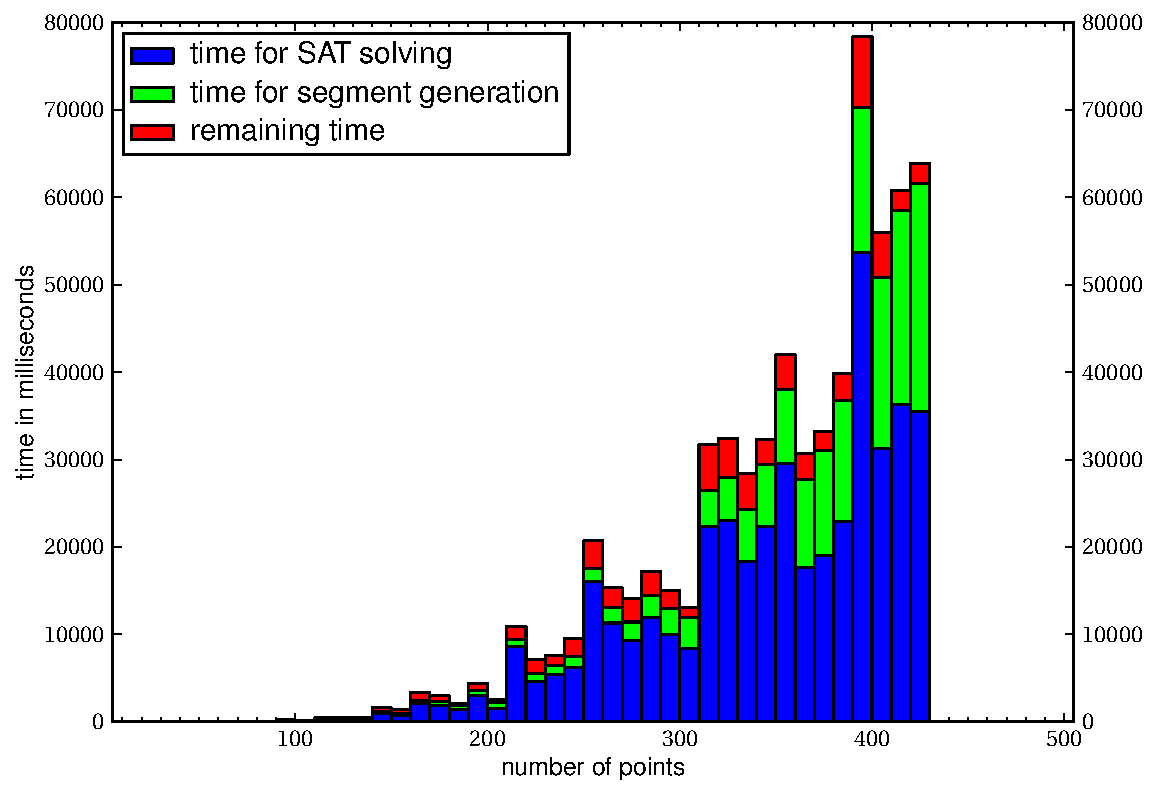
\includegraphics[width=\linewidth,height=\textheight,keepaspectratio]{results/time_comparison.pdf}
  \caption{\label{fig:time_comparison}Comparison of execution times}
\end{figure}

\begin{figure}[ht]
  \centering
  \thisfloatpagestyle{empty}
  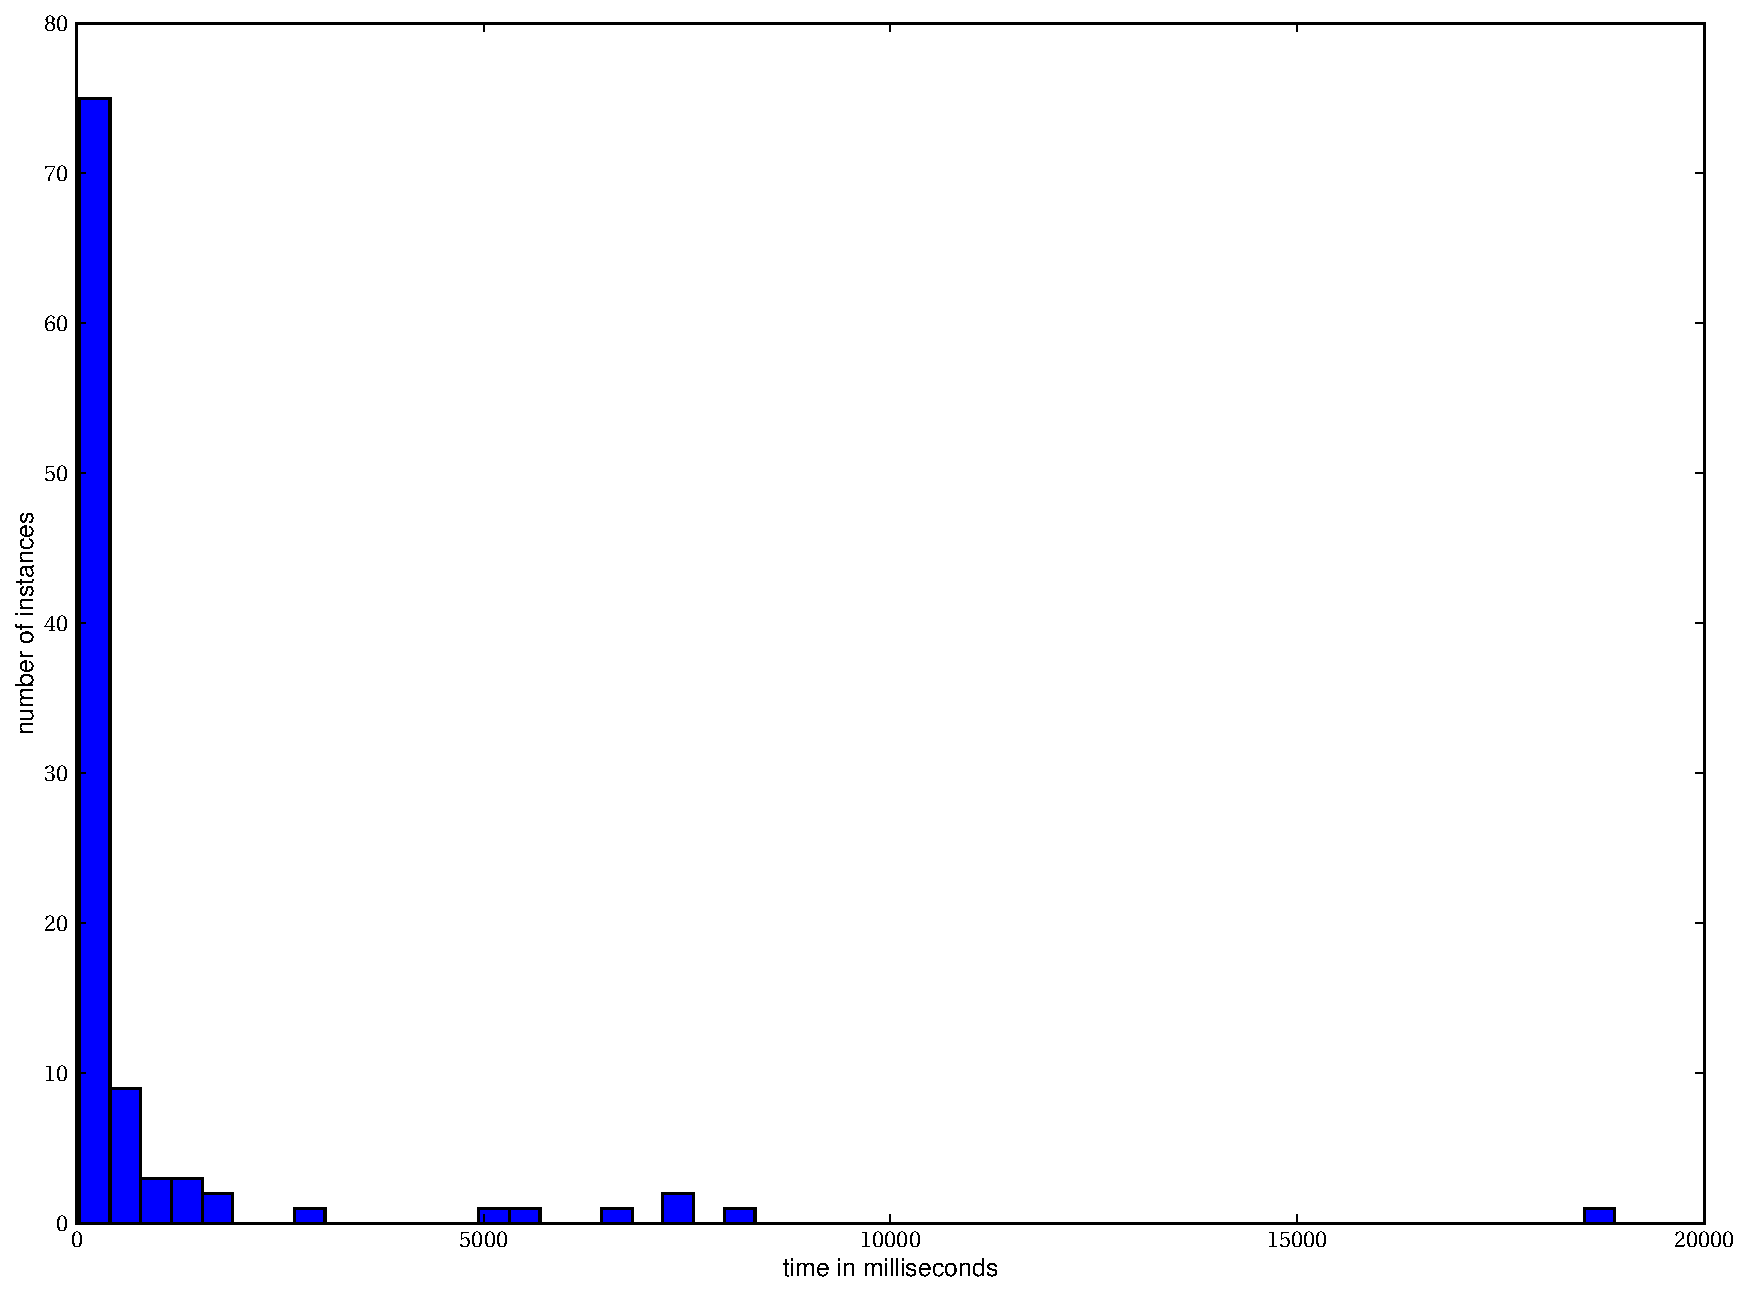
\includegraphics[width=\linewidth,height=\textheight,keepaspectratio]{results/time_hist_70.pdf}
  \caption{\label{fig:times_70}Histogram of execution times for 70 points}
\end{figure}

\begin{figure}[ht]
  \centering
  \thisfloatpagestyle{empty}
  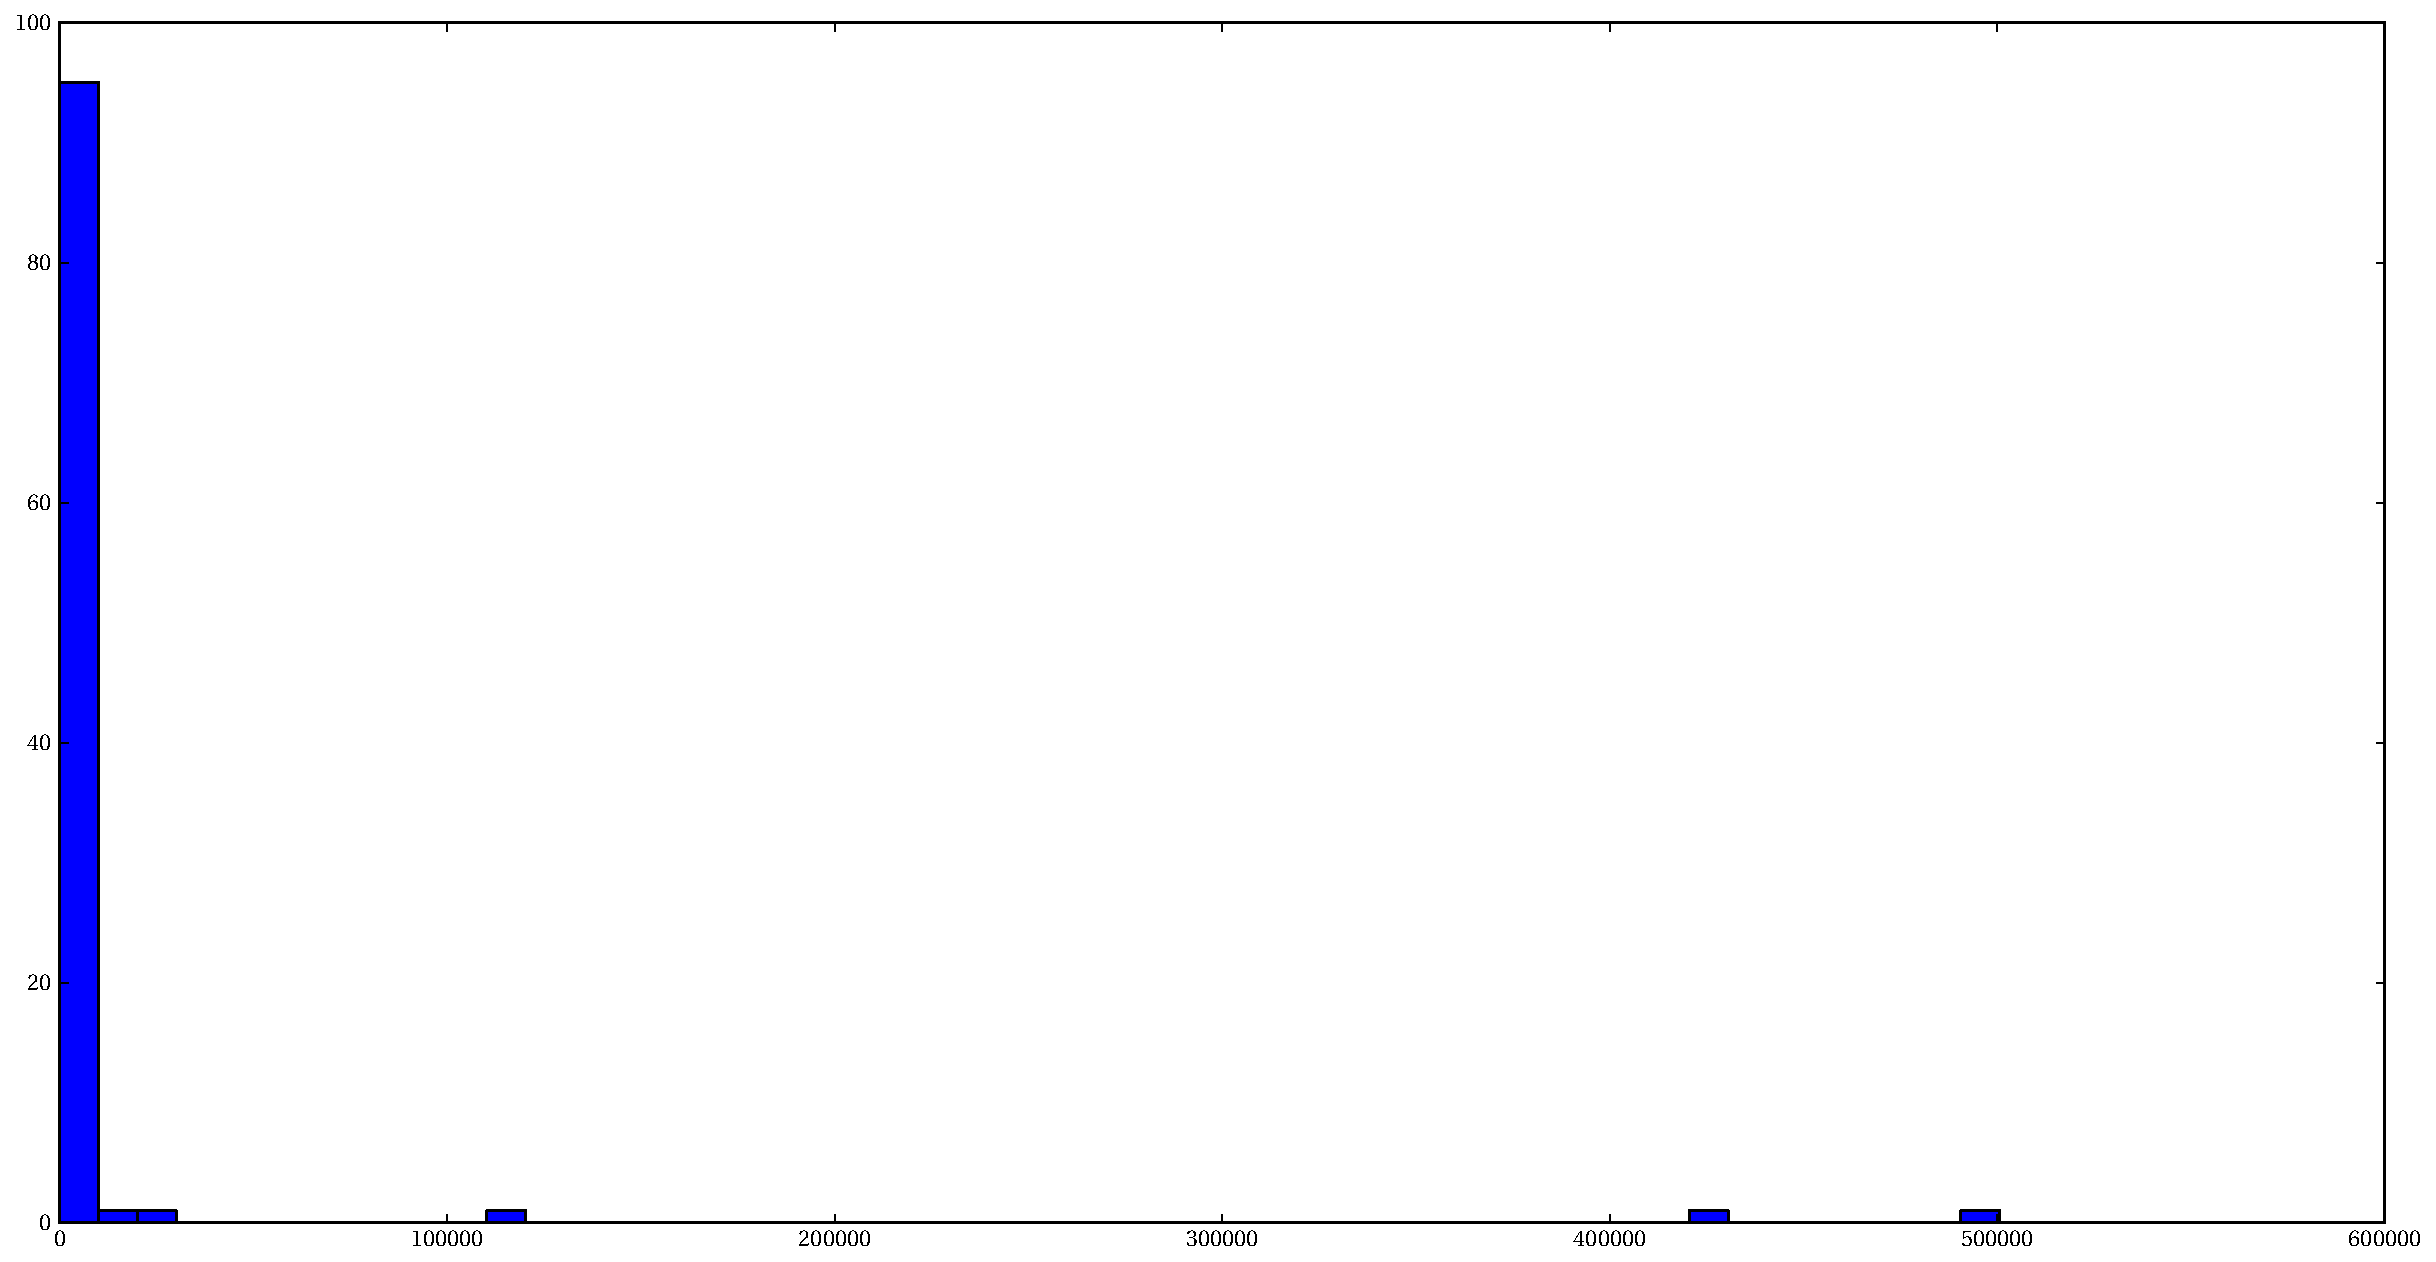
\includegraphics[width=\linewidth,height=\textheight,keepaspectratio]{results/time_hist_80.pdf}
  \caption{\label{fig:times_80}Histogram of execution times for 80 points}
\end{figure}
\end{landscape}
\restoregeometry

\section{Aborted instances}

\newgeometry{margin=1.5cm}
\begin{landscape}
\begin{figure}[ht]
  \centering
  \thisfloatpagestyle{empty}
  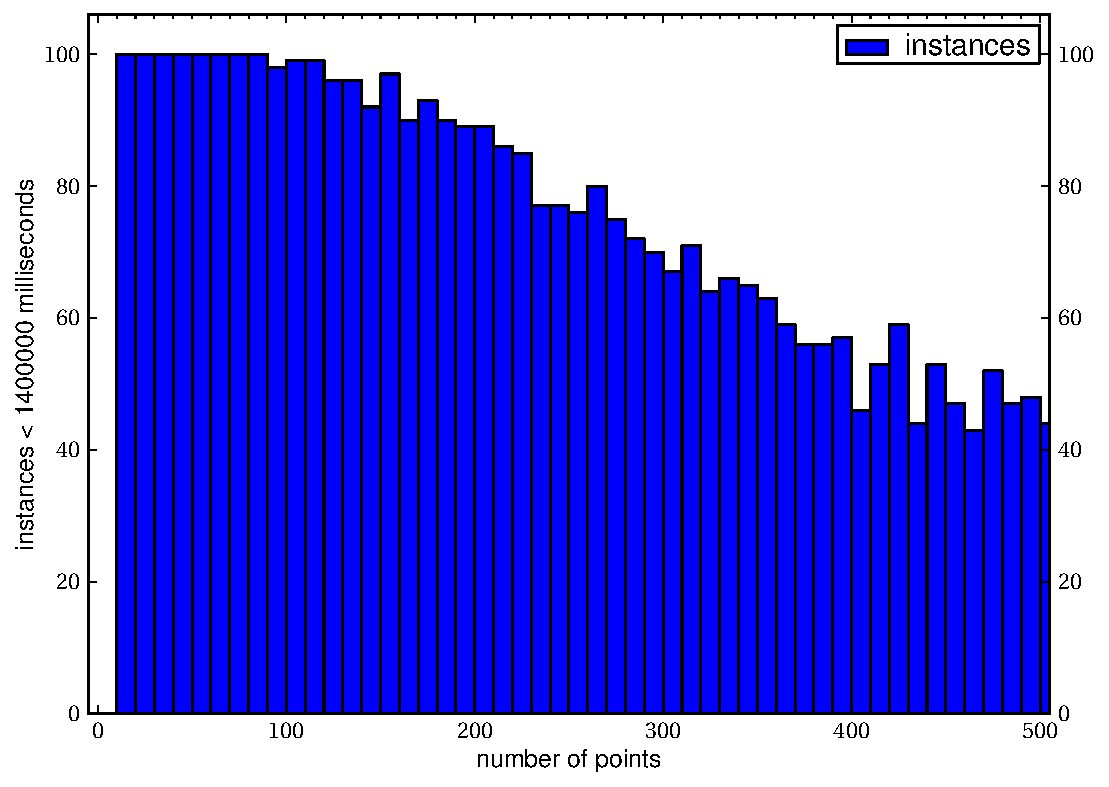
\includegraphics[width=\linewidth,height=\textheight,keepaspectratio]{results/time_hist.pdf}
  \caption{\label{fig:times_hist}Histogram of finished instances}
\end{figure}

\begin{figure}[ht]
  \centering
  \thisfloatpagestyle{empty}
  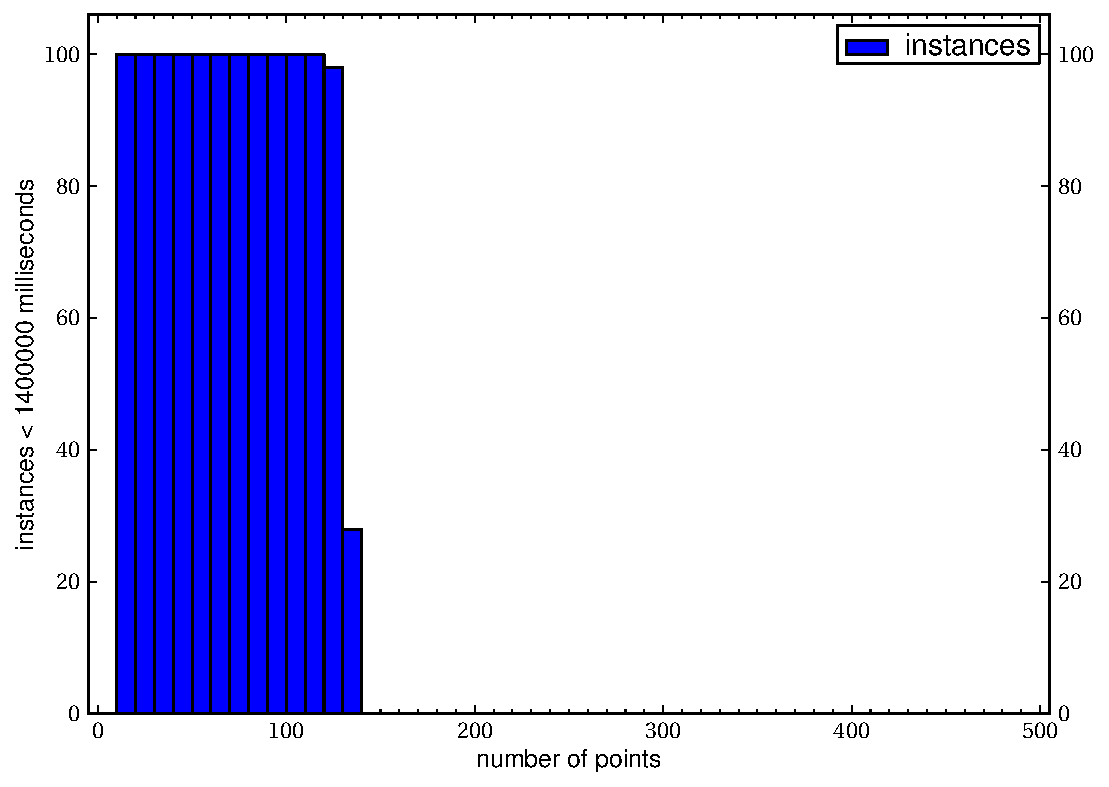
\includegraphics[width=\linewidth,height=\textheight,keepaspectratio]{results/complete_sat/time_hist.pdf}
  \caption{Histogram of finished instances (complete SAT)}
\end{figure}
\end{landscape}
\restoregeometry
